\section{Análisis tecnológico}


\subsection{Fundamentos de una skill}

Qué es una skill

\subsubsection{Términos comunes en el desarrollo de skills}

intents

utterances

handlers 

slots

\subsubsection{Memoria y persistencia de datos}

session attributes y DynamoDB entre sesiones.

\subsection{Alexa Skills Kit (ASK)}

ASK es un conjunto de APIs y herramientas que facilitan la integración de nuevas habilidades en Alexa, permitiendo crear distintas clases de skills, desde personalizadas hasta otras específicas para vídeo, listas y hogar inteligente.

El tipo de skill que mejor se ajusta a los objetivos preestablecidos es la personalizada o \textit{Custom Skill}, pues esta permite más flexibilidad a los desarrolladores, permitiéndoles adaptarla a las necesidades de la aplicación a desarrollar.

Se puede importar ASK, a través del nombre de la biblioteca: \textit{ask-sdk-core}.

\subsection{AWS Serverless Platform}

Para el desarrollo de skills de Alexa, se puede optar o bien por la función Lambda de AWS, o bien por un servicio web distinto. La primera opción pertenece a un conjunto de herramientas de desarrollador y servicios en la nube de alto rendimiento que componen la Plataforma sin Servidor de AWS.

Se va a utilizar \textbf{AWS Lambda} para la creación de este juego digital, aprovechando así las múltiples funcionalidades y material de apoyo para encaminar el proceso de desarrollo. Además, al poder hacer uso de los otros servicios incluidos en esta plataforma (DynamoDB, Amazon S3, etc), se garantiza cierta centralización y absoluta compatibilidad entre ellos.

\subsection{Alexa Presentation Language (APL)}

La parte visual de la skill se gestiona mediante el lenguaje de presentación de Alexa (APL), a través del envío de documentos APL al dispositivo en forma de una directiva que se verá más adelante.

Un documento APL consiste en un fichero JSON que define la estructura y disposición de elementos a mostrar por la pantalla del dispositivo de Alexa.
A continuación se muestra un ejemplo básico de documento APL que imprime por pantalla una cadena de texto:

\begin{figure}[H]
	\centering
	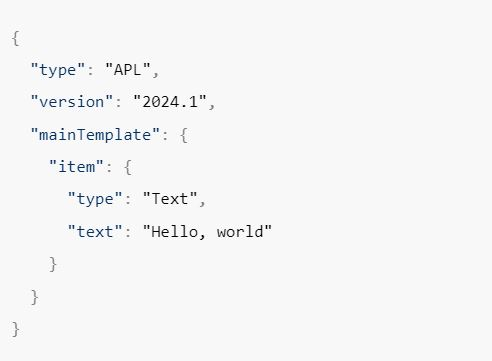
\includegraphics[width=0.6\textwidth]{imgs/apl-example.JPG}
	\caption{Ejemplo de documento APL básico (\href{https://developer.amazon.com/en-US/docs/alexa/alexa-presentation-language/apl-document.html}{Alexa Developer Documentation})}
	\label{fig:apl-ejemplo}
\end{figure}

